%!TEX root = ../paper.tex

%%%%%%%%%%%%%%%%%%%%%%
\section{Why Do Programmers Do Code Reviews?} \label{sec:expectations}
%%%%%%%%%%%%%%%%%%%%%%


Our first research question seeks to understand what motivations and
expectations drive code reviews, and whether managers and developers share the
same opinions.

Based on the responses that we coded from observations of developers performing
code review as well as interviews, there are various motivations for code
review. Overall, the interviews revealed that finding defects, even though
prominent, is just one of the many motivations driving developers to perform
code reviews. Especially when reinforced by a strong team culture around
reviews, developers see code reviews as an activity that has multiple
beneficial influences not only on the code, but also for the team and the
entire development process. In this vein, one senior developer's comment
summarized many of the responses: \quotation{{\normalfont[code review]} also has several
beneficial influences: \begin{inparaenum}[(1)]
\item makes people less protective about their code, 
\item gives another person insight into the code, so there is 
\item better sharing of information across the team, 
\item helps support coding conventions on the team,
and {\normalfont[...]}
\item helps improving the overall process and quality of code.
\end{inparaenum}}

Through the card sort on both meetings and code review comments, we found
several references to motivations for code review and identified six main
topics. To complete this list, in the survey for managers, we included an open
question on why they perform code reviews in their team. We analyzed the
responses to create a comprehensive list of high-level motivations. We included
this list in the developers' survey and asked them to rank the top three main
reasons that described why they do code reviews.

In the rest of this section, we discuss the motivations that emerged as the
most prominent. We order them according to the importance they were given by
the 873 developers and testers who responded to the final survey.

\subsection{Finding Defects}

One interviewed senior tester explains that he performs code reviews because
they \quotation{are a great source of bugs;} he goes even further stating:
\quotation{sometimes code reviews are a cheaper form of bug finding than
testing.} Moreover, the tool seems not to have an impact on this main
motivation: \quotation{using CodeFlow or using any other tool makes a little
difference to us; it's more about being able to identify flaws in the logic.}

Almost all the managers included \emph{finding defects} as one of the reasons for
doing code reviews; for 44\% of the managers, it is the top reason. Managers
considered defects to be both low level issues (\eg \quotation{correct logic
is in place}) and high level concerns (\eg \quotation{catch errors in
design}). Concerning surveyed developers/testers, \emph{finding defects} is the
first motivation for code review for 383 of the programmers (44\%), second
motivation for 204 (23\%), and third for 96 (11\%).

This is in-line with the reason why code inspections were devised in the first
place: reducing software defects~\cite{ackerman1984software}.

Nevertheless, even though \emph{finding defects} emerged from our data as a strong
motivation (the first for almost half of the programmers and managers),
interviews and survey results indicate that this only tells part of the story
of why practitioners do code reviews and the outcomes they expect.

\subsection{Code Improvement}

Code improvements are comments or changes about code in terms of readability,
commenting, consistency, dead code removal, \etc, but do not involve
correctness or defects.

Programmers ranked \emph{code improvement} as an important motivation for code
review, close to \emph{finding defects}: This is the primary motivation for 337~(39\%)
programmers, the second for 208~(24\%), and the third for 135~(15\%).
Managers reported \emph{code improvement} as their primary motivation in 51~(31\%) cases. One manager wrote how code review in her view is a
\quotation{discipline of explaining your code to your peers {\normalfont[that]} drives a
higher standard of coding. I think the process is even more important than the
result.}

Most interviewed programmers mentioned that at least one of the reviewers
involved in each code review takes care of checking whether the code follows
the team conventions, for example in terms of code formatting and in terms of
function and variable naming. Some programmers use a ``code improvement''
check as a first step when doing code review: \quotation{the first basic pass
on the code is to check whether it is standard across the team.}

The interviews also gave us a glimpse of the connection between the quality of
code reviews and code improvement comments. Such comments seem easier to
write and sometimes interviewees mentioned them as the way reviewers use to
avoid spending time to conduct good code reviews. An observation by a senior
developer, in the company for more than nine years, summarizes the opinions we
received from many interviewees: \quotation{I've seen quite a few code reviews
where someone commented on formatting while missing the fact that there were
security issues or data model issues.}

\begin{figure}[t] %  figure placement: here, top, bottom, or page
   \centering
   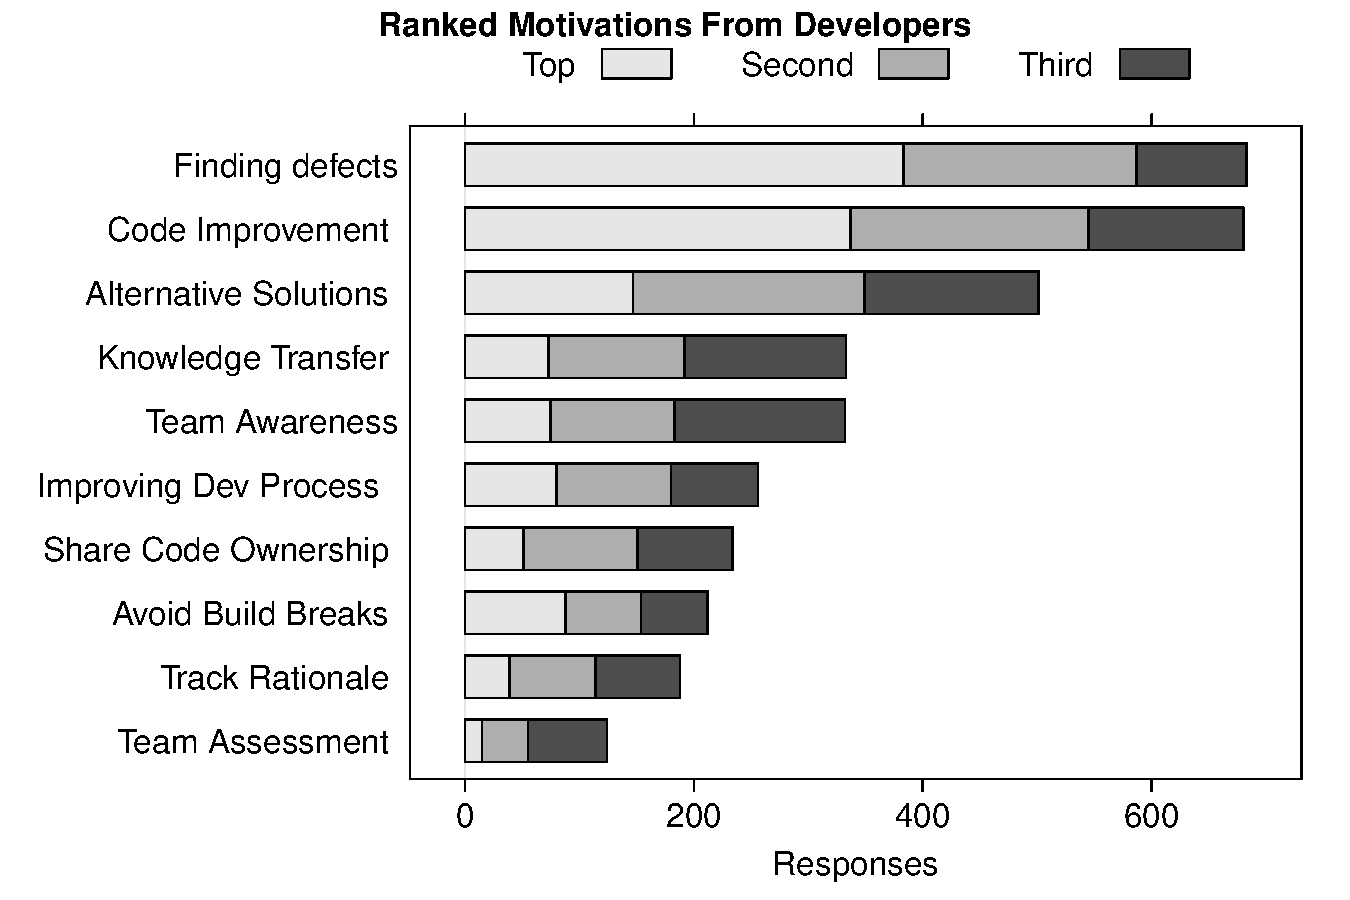
\includegraphics[width=\columnwidth]{dev_motivations.pdf}
   \vspace{-1.5em}
   \caption{Developers' motivations for code review.}
   \label{fig:dev-motivations}
   \vspace{-1.5em}
\end{figure}


\subsection{Alternative Solutions}

\emph{Alternative solutions} regard changes and comments on improving the
submitted code by adopting an idea that leads to a better implementation. This
is one of the few motivations in which developers and managers do not agree.
While 147~(17\%) developers put this as the first motivation, 202~(23\%) as the
second, and 152~(17\%) as the third, only 4~(2\%) managers even mentioned it
(\eg \quotation{Generate better ideas, alternative approaches} and
\quotation{Collective wisdom: Someone else on the project may have a better
idea to solve a problem}). The outcome of the interviews was similar to the
position of managers: Interviewees vaguely mentioned this motivation, and
mostly in terms of generic \quotation{better ways to do things.}


\subsection{Knowledge Transfer}

All the interviewees but one motivated their code reviews also from a learning---or \emph{knowledge transfer}---perspective. With the words of a senior developer:
\quotation{one of the things that should be happening with code reviews over
time is a distribution of knowledge. If you do a code review and did not learn
anything about the area and you still do not know anything about the area, then
that was not as good code review as it could have been.} Although we did not
include questions related to \emph{knowledge transfer} in our interview guideline,
this topic kept emerging spontaneously from each meeting, thus underscoring its
value for practitioners.

Sometimes programmers told us that they follow code reviews explicitly for
learning purposes. For example, a tester explained: \quotation{{\normalfont[I read code
reviews because]} from a code review you can learn about the different parts you
have to touch to implement a certain feature.}

According to interviewees, code review is a learning opportunity for both the
author of the change and the reviewers: There is a bidirectional knowledge
transfer about APIs usage, system design, best practices, team conventions,
\quotation{additional code tricks,} \etc Moreover code reviews are recognized
for educating new developers about code writing.

Managers included \emph{knowledge transfer} as one of the reasons for code review,
although never as the top motivation. They mostly wrote about code review as an
education means by mentioning among the motivations:
\quotation{developer education,} \quotation{education for junior developers who
are learning the codebase,} and \quotation{learning tool to teach more junior
team members.}

Programmers answering the survey declared \emph{knowledge transfer} to be their
first motivation for code review in 73~(8\%) cases, their second in 119~(14\%),
and their third in 141~(16\%).

\subsection{Team Awareness and Transparency}

During one of our observations, one developer was preparing a code review
submission as an author: He wanted other developers to \quotation{double check}
his changes before committing them to the repository. After preparing the code,
he specified the developers he wanted to review his code; he required not only
two specific people, but he also put a generic email distribution group as an
\quotation{optional} reviewer. When we inquired about this choice, he explained
us: \quotation{I am adding {\normalfont[this alias]}, so that everybody {\normalfont[in the team]} is
notified about the change I want to do before I check it in.} In the subsequent
interviews, this concept of using an email list as optional reviewer, or
including specific optional reviewers exclusively for awareness emerged again
frequently, \eg \quotation{Code reviews are good FYIs {\normalfont[for your
information]}.}

Managers often mentioned the concept of team awareness as a motivation for code
review, frequently justifying it with the notion of ``transparency:'' Not only
must the team be kept aware of the directions taken by the code, but also
nobody should be allowed to ``secretly'' make changes that might break the code
or alter functionalities.

The 873 programmers answering the survey ranked \emph{team awareness and
transparency} very close to \emph{knowledge transfer}. In fact, the two concepts
appeared logically related also in the interviews; for example one tester,
while reviewing some code said: \quotation{oh, this guy just implemented this
feature, and now let me back and use it somewhere else.} Showing that he both
learned about the new feature and he was now aware of the possibility to use it
in his own code. 75~(9\%) developers considered team awareness their first
motivation for code review, 108~(12\%) their second, and 149~(17\%) their
third. 

Although \emph{team awareness and transparency} emerged from our data as clearly
promoted by the code review process, academic research seems to have given
little attention to it. 

\subsection{Share Code Ownership}

The concept of \emph{shared code ownership} is closely related to \emph{team awareness
and transparency}, but it has a stronger connotation toward active
collaboration and overlapping coding activities. Programmers and managers
believe that code review is not only an occasion to notify other team members
about incoming changes, but also a means to have more than one knowledgeable
person about specific parts of the codebase. A manager put the following as her
second motivation for code review: \quotation{Broaden knowledge \& understanding
of how specific features/areas are designed and implemented (e.g., grooming
``backup developers'' for areas where knowledge is too concentrated on one or
two expert developers).}

Moreover, both developers and managers have the opinion that practicing code
review also improves the personal perception of team members about shared code
ownership. On this note, a senior developer, with more than 30 years in the
software industry, explained: \quotation{In the past people did not use to do
code reviews and were very reluctant to put themselves in positions where they
were having other people critiquing their code. The fact that code reviews are
considered as a normal thing helps immensely with making people less protective
about their code.} Similarly a manager wrote us explaining that she deems code
reviews important because they \quotation{Dilute any ``rigid sense of
ownership'' that might develop over chunks of code.}

In the programmers' survey, 51~(6\%) respondents marked \emph{share code
ownership} as their first motivation, 100~(11\%) as their second, and 91~(10\%)
as their third.

\subsection{Summary}

In this section, we analyzed the motivations that developers and managers have
for doing code review. We abstracted them into a list, which we finally
included in the programmers' survey. Figure 3 reports the answers given to this
question: The black bar is the number of developers that put that row as their
top motivation, the gray bar is the number that put it as the second
motivation, \etc We have ordered the factors by giving 3 points for a first
motivation response, 2 points for a second motivation, \etc and then sorting by
the sum. 

We discussed the five most prominent motivations, which show that \emph{finding
defects} is the top motivation, although participants believe that code review
brings other benefits. The first two motivations were already popular in
research and their effectiveness have been evaluated in the context of code
inspections; on the contrary, the other motivations are still unexplored,
especially those regarding more social benefits on the team, such as shared
code ownership.

Although motivations are well defined, we still have to verify whether they
actually translate into real outcomes of a modern code review process. 
